\documentclass{article}
\usepackage{graphicx,spconf,amsmath,amssymb,subfigure,color,hyperref}
\definecolor{darkgreen}{rgb}{0,0.5,0}
\newcommand{\Ntrg}{\big[N_{p=1, m=1} + \lambda \big] + \big[N_{p=1, m=2} + \lambda \big] + \ldots + \big[N_{p=1, m=M} + \lambda \big]}
\newcommand{\jointcnt}{\sum\limits_{n_{trg}=1}^{N_{trg}}I(X_p=x_p, X_{P-1}=x_{P-1})}
\newcommand{\singlecnt}{\sum\limits_{n_{trg}=1}^{N_{trg}}I(X_{P-1}=x_{P-1})}
\newcommand{\singlep}{p(X_{P-1}=x_{P-1})}
\newcommand{\singlepone}{p(X_{P-1}=1)}
\newcommand{\singleptwo}{p(X_{P-1}=2)}
\newcommand{\singlepM}{p(X_{P-1}=M)}
\newcommand{\condp}{p(X_p=x_p | X_{P-1}=x_{P-1})}
\newcommand{\jointp}{p(X_p=x_p, X_{P-1}=x_{P-1})}
\newcommand{\KmeansOuterSum}{\sum\limits_{k=1}^K}
\newcommand{\KmeansInnerSum}{\sum\limits_{{i=1 \atop x_i \in \mathcal{C}_k}}^N}
\newcommand{\KmeansSum}{\KmeansOuterSum \KmeansInnerSum}
\newcommand{\RVQInnerSum}{\sum\limits_{{i=1 \atop g_i \mapsto m_{\rho, s}}}^N}
\newcommand{\RVQOuterSum}{\sum_{m=1}^M}
\newcommand{\RVQsum}{\KmeansOuterSum \sum\limits_{{i=1 \atop g_i \in \mathcal{H}_k}}^N}
\newcommand{\KmeansInner}{{(x_i - y_k)}^2}
\newcommand{\RVQinner}{            {(x_i  - \hat{\mu}^{(k)})}^2}
\newcommand{\RVQinneralternate}{{(g_i - \mu_\rho^{(k)})}^2}
\newcommand{\RVQinneralternatealternate}{{(g_i - m_{\rho, s})}^2}
\newcommand{\KmeansError}{\KmeansSum \KmeansInner}
\newcommand{\RVQerror}     {\KmeansSum \RVQinner}
\newcommand{\RVQerroralternate}{\RVQsum \RVQinneralternate}
\newcommand{\RVQunit}{x_i -\bigg(\sum_{p=1}^P\mu^{(k)}_p\bigg)}
\newcommand{\RVQequivalentCodevector}{\sum_{p=1 }^P\mu^{(k)}_p}
\newcommand{\RVQequivalentCodevectorBroken}{\sum_{p=1 \atop p \neq \rho}^P\mu^{(k)}_p+ \mu^{(k)}_\rho}
\newcommand{\RVQmultipleKmeans}{x_i -\bigg(\RVQequivalentCodevectorBroken\bigg)}
\newcommand{\RVQmultipleKmeansone}{x_i -\bigg(\sum_{p=2}^P\mu^{(k)}_p+ \mu^{(k)}_\rho\bigg)}
\newcommand{\RVQmultipleKmeansonealternate}{\bigg(x_i -\sum_{p=1 \atop p \neq \rho}^P\mu^{(k)}_p\bigg) - \mu^{(k)}_\rho}
\newcommand{\RVQmultipleKmeanstwo}{x_i -\bigg(\sum_{p=1 \atop p \neq 2}^P\mu^{(k)}_p+ \mu^{(k)}_\rho\bigg)}
\newcommand{\RVQmultipleKmeansT}{x_i -\bigg(\sum_{p=1}^{P-1}\mu^{(k)}_p+ \mu^{(k)}_\rho\bigg)}
\newcommand{\EucMatrix}
{
\left[
\begin{array}{lll}
r_{11} & r_{12} & t_x \\ 
r_{21} & r_{22} & t_y \\ 
0 & 0 & 1 \\ 
\end{array}
\right]
}	

\newcommand{\SimMatrix}
{
\left[
\begin{array}{lll}
sr_{11} & sr_{12} & t_x \\ 
sr_{21} & sr_{22} & t_y \\
0 & 0 & 1 \\ 
\end{array}
\right]
}

\newcommand{\AffMatrix}
{
\left[
\begin{array}{lll}
a &b & t_x \\ 
c & d & t_y \\
0 & 0 & 1 \\
\end{array}
\right]
}

\newcommand{\ProjMatrix}
{
\left[
\begin{array}{lll}
h_{11} & h_{12} & h_{13} \\ 
h_{21} & h_{22} & h_{23} \\ 
h_{31} & h_{32} & h_{33} \\ 
\end{array}
\right]
}

\newcommand{\RotMatrixTheta}
{
\left[
\begin{array}{rr}
\cos(\theta) & -\sin(\theta) \\ 
\sin(\theta) & \cos(\theta) \\ 
\end{array}
\right]
}

\newcommand{\RotMatrixPhi}
{
\left[
\begin{array}{rr}
\cos(\phi) & -\sin(\phi) \\ 
\sin(\phi) & \cos(\phi) \\ 
\end{array}
\right]
}

\newcommand{\RotMatrixminusPhi}
{
\left[
\begin{array}{rr}
\cos(-\phi) & -\sin(-\phi) \\ 
\sin(-\phi) & \cos(-\phi) \\ 
\end{array}
\right]
}


\newcommand{\EigenvalueMatrix}
{
\left[
\begin{array}{cc}
\lambda_1 & 0\\
0 & \lambda_2
\end{array}
\right]
}

\newcommand{\bigMatrix}
{
s \left[
\begin{array}{cc}
 (r)(a) + b &  (r)(d) - c \\
 (r)(c) - d &  (r)(b) + a
\end{array}
\right]
}


\newcommand{\bigMatrixTwo}
{
\left[
\begin{array}{cc}
(\lambda_2) p + (\lambda_1) q & (\lambda_2) s  - (\lambda_1) r \\
(\lambda_2) r  - (\lambda_1) s & (\lambda_2) q + (\lambda_1) p
\end{array}
\right]
}
\newcommand{\dr}{(\mathbf{x}_i-\boldsymbol\mu_k)^T(\mathbf{x}_i-\boldsymbol\mu_k) + \lambda({P_{\textrm{max}}-P_i})}

\title{TARGET TRACKING USING RESIDUAL VECTOR QUANTIZATION}
\twoauthors
 {Salman Aslam}	
{National University of Sciences and Technology \\Islamabad, Pakistan}	
  {Christopher Barnes, Aaron Bobick}
	{Georgia Institute of Technology\\
	Atlanta, USA}
\begin{document}
\ninept
\maketitle
\begin{abstract}
In this work, our goal is to track visual targets using residual vector quantization (RVQ).  We compare our results with principal components analysis (PCA) and tree structured vector quantization (TSVQ) based tracking.  This work is significant since PCA is commonly used in the Pattern Recognition, Machine Learning and Computer Vision communities. On the other hand, TSVQ is commonly used in the Signal Processing and data compression communities. RVQ with more than two stages has not received much attention due to the difficulty in producing stable designs. In this work, we bring together these different approaches into an integrated tracking framework and show that RVQ tracking performs best according to multiple criteria over a variety of publicly available datasets. Moreover, an advantage of our approach is a learning-based tracker that builds the target model while it tracks, thus avoiding the costly step of building target models prior to tracking.
\end{abstract}
%
\begin{keywords}
Residual vector quantization, tracking, RVQ, PCA, TSVQ, learning, generalization
\end{keywords}

%--------------------------------------------------------------------------------------------------------------------------------------------------------------
\section{INTRODUCTION}
%--------------------------------------------------------------------------------------------------------------------------------------------------------------
Visual tracking is the task of estimating a target's state over time.  In many cases, the "target state" can be defined to represent target position, a bounding box around the target, or the target contour.  (see~\cite{2006_JNL_SURVEYtrk_Yilmaz} for several possible target representations).  Tracking is a challenging problem due to appearance, contour and pose changes, warping, self occlusion, motion blur, structured and random noise, non-symmetic BRDF, lighting changes, sudden target or camera motion, motion blur, and target exits and merges.  Traditional trackers overcome these challenges using point, region or contour based tracking.  Recently, trackers that try to learn the appearance of the target, either in offline or online mode have been introduced~\cite{2004_JNL_SVMtracking_Avidan, 2008_JNL_subspaceTRK_Ross}.  In this work, we use the latter approach of online learning in a single-target tracking framework.  

Seminal work in this area can be traced back to 1996 when Black and Jepson experimented with tracking using an eigenspace representation of the target appearance model~\cite{1998_JNL_Eigentracking_Black}.  The next notable work is by Moghaddam and Pentland in 1997~\cite{1997_JNL_EigenTRK_Moghaddam} in which they try to address a fundamental limitation of PCA: 2 different vectors, $\mathbf{x}_1$ and $\mathbf{x}_2$ can have the same distance to a reduced eigenspace, i.e., projection error $\mathbf{e}_1$ and $\mathbf{e}_2$ respectively, even if they have different distance to the mean $\boldsymbol\mu$ of the data that was used to create the eigenspace.  They formulate the problem using DIFS (distance in feature space) and DFFS (distance from feature space) so that both projection error and within-subspace distance to the mean of the data are used while trying to determine how well the subspace explains a new data-point.  The next breakthrough came with the work of Bishop and Tipping in 1999~\cite{1999_JNL_PPCA_Tipping}, where they show that a probabilistic variation of PCA, probabilistic PCA (PPCA), allows PCA to be used as a generative model.  The advantage in tracking is that this methodology allows an assignment of probabilities to new data-points and therefore allows relative weighting of track candidates.  Ideas from these three works were combined into a tracking framework by Ross et. al. in 2008~\cite{2008_JNL_subspaceTRK_Ross}.  Moreover, they used incremental SVD to make their tracker run in real time.  

Here, we extend this work by Ross et. al. using RVQ in a similar tracking framework and comparing it with PCA and TSVQ based tracking.  We also introduce four methods for relative weighting of track candidates for RVQ.  The result is a generative framework for RVQ that leads to robust tracking.  Whereas RVQ was first introduced by Juang and Gray in 1982~\cite{1982_CNF_SpeechRVQ_JuangGray}, and subsequently extended by Barnes~\cite{1996_JNL_AdvancesRVQ_Barnes,2007_JNL_IDDM_Barnes}, this algorithm has received little attention outside the signal processing and data compression communities.  In this work, our goal is to introduce the clustering-based RVQ algorithm in the computer vision and machine learning fields where a much simpler cluster-means (K-means) based classifier has been widely used~\cite{2008_JNL_PRML_Wu}.  We present RVQ in the context of an important and challenging problem, that of visual target tracking.  The next two sections therefore present an overview of RVQ and visual tracking.

%Before we proceed, a few definitions are introduced.

								\begin{figure}[t]
								\centering	
								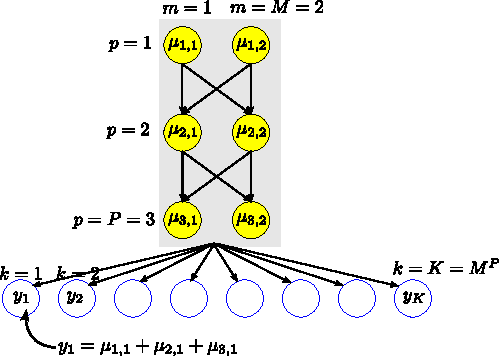
\includegraphics[width=0.35\textwidth]{figs/RVQ_trellis}
								\caption{RVQ $\sigma$-tree, 3 stages, 2 code-vectors per stage, i.e., $P$=3, $M=2$.  This is a 3x2 $\sigma$-tree.} 
								\label{fig:RVQ_sigma_tree}				
								\end{figure}

%\begin{enumerate}
%\item \underline{Quantization}.  Quantization is the process of representing a large, possibly infinite, set of values with a smaller set of values~\cite{2005_BOOK_DataCompression_Sayood}.  For a quantizer $\mathcal{Q}$ that takes values from a source alphabet $\mathcal{X}=\{\mathbf{x} \in \mathbb{R}^D\}$ and maps them to a reconstruction alphabet $\mathcal{C}=\{\mathbf{y}_k \in \ \mathbb{R}^D \ | \ k=1,2, \ldots K\}$.  If the input is scalar, i.e. $D=1$, the quantizer is called a \emph{scalar quantizer}.  For $D>1$, the quantizer is called a \emph{vector quantizer}.  Quantization is used widely for achieving lossy compression in images and videos.  For instance, all current video standards, MPEG-1, MPEG-2, MPEG-4, H.261, H.263 and H.264 rely on a special form of quantization called \emph{transform vector quantization}. 
%
%\item \underline{Encoding}.  During this process, the input $\mathbf{x}$ to be quantized is represented by an index $m$, usually a scalar, that corresponds to the code-vector $\mathbf{y}_k$ that $\mathbf{x}$ is mapped to.
%
%\item \underline{Decoding}.  During this process, the index $m$ is used to look up code-vector $\mathbf{y}_k$.  
%
%\item \underline{Parititions}.  Quantization creates $K$ partitions $\mathcal{P}_k = \{\mathbf{x} \ \in \ \mathbb{R}^D \ | \ \mathcal{Q}(\mathbf{x}) = \mathbf{y}_k\}$ in the input space $\mathbb{R}^D$ which are mutually exclusive and exhaustive, i.e., $\mathcal{P}_i \bigcap \mathcal{P}_j = \emptyset, \ i \neq j$.  The union of these partitions covers the entire input space, $\bigcup\limits_{k=1}^{K} \mathcal{P}_k=\mathbb{R}^D$.
%
%\item \underline{Codebook}. The reconstruction alphabet $\mathcal{C}$ is known as the \emph{codebook}.  
%
%\item \underline{Code-vectors}.  The $K$ members $\mathbf{y}_k$ of the reconstruction alphabet $\mathcal{C}$ are called \emph{code-vectors}.  The term \emph{centroid} is used interchangeably with code-vector.
%
%\item \underline{Design-time}.  In the context of quantization, design-time refers to the process of generating the codebook.
%
%\item \underline{Run-time}.  In the context of quantization, run-time refers to the process of mapping an input $\mathbf{x}$ to a code-vector $\mathbf{y}$, i.e., the process of encoding followed by the process of decoding.
%
%\item \underline{Rate}.  If we have $K$ code-vectors $\mathbf{y}_k$ in $\mathbb{R}^D$, $\log_2 K$ bits are required to represent each code-vector.   The \emph{resolution}, \emph{code rate}, or simply the \emph{rate} $r$ of a quantizer is the number of bits required to represent each sample, i.e., scalar element of $\mathbf{y}_k$.  Since there are $D$ samples, the rate $r=\frac{\log_2 K}{D}$.  
%
%\item \underline{Distortion}.  The difference between original input $\mathbf{x}$ and reconstructed output $\hat{\mathbf{x}}~=~\mathcal{Q}~(\mathbf{x})~=~\mathbf{y}$ is known as \emph{distortion} $d(\mathbf{x}, \mathbf{y})$~\cite{2005_BOOK_DataCompression_Sayood}.  A commonly used distortion measure is the squared error criterion, $d(\mathbf{x}, \mathbf{y})=(\mathbf{x}-\mathbf{y})^2$.  Average distortion is given by $e(\mathcal{X}, \mathcal{C})~=~\mathrm{E}\left[d(\mathbf{x}, \mathbf{y}) \right]$.  
%

%
%\item \underline{Quantization optimality}.  A widely used algorithm to compute at least locally optimal codevectors and partitions is the Generalized Lloyd Algorithm (GLA)~\cite{1991_BOOK_VQ_GershoGray}, also known as the Linde Buzo Gray (LBG) algorithm~\cite{1982_JNL_LeastSquaresQuantization_Lloyd} or K-means clustering~\cite{1967_CNF_Kmeans_Macqueen}.  Scalar quantization case for an input $X$ with distribution $f_X(x)$ and average distortion $e$, is given by, $e= \int\limits_{-\infty}^\infty(x - \hat{x})^2f_X(x)dx=\sum\limits_{k=1}^K \int\limits_{b_k}^{b_{k+1}}(x-y_k)^2f_X(x)dx$.
%
%If the partition $\mathcal{P}_k = \left\{x \ | \ (y_k-x)^2 < (y_j-x)^2, \ \forall \ j \neq k \right\}$ is given, the optimal code-vector $y_k$ for this partition can be computed by setting the derivative of the average distortion $e$ with respect to $y_k$ equal to 0, i.e., $\frac{\partial{e}}{\partial{y_k}} = 0$.  Solving for $y_k$, we get $y_k = \frac{\int\limits_{b_k}^{b_{k+1}}xf_X(x)dx}{\int\limits_{b_k}^{b_{k+1}}f_X(x)dx}$.  In other words, the optimal centroid for a given partition and the squared error criterion is the centroid of the partition.
%
%\item \underline{RVQ sigma ($\sigma$) tree}.  An RVQ $\sigma$-tree is shown in Figure~\ref{fig:RVQ_sigma_tree}.  Each node of this tree, $\mu_{m,p}$ is called a \emph{stage code-vector} and is the $m$-th node at the $p$-th stage.  There are a total of $M$ code-vectors in each of the $P$ stages.  In Figure~\ref{fig:RVQ_sigma_tree}, there are 6 stage-code-vectors, 2 at the first stage, 2 at the second stage, and 3 at the third stage.  The leaf nodes of this tree, also called \emph{equivalent code-vectors}~\cite{2007_JNL_IDDM_Barnes} constitute the RVQ code-book~\cite{2002_JNL_SigmaTrees_Barnes}.  Each equivalent code-vector is created using a \emph{direct sum}, i.e., by adding one stage code-vector from each stage.  There are $K=M^P$ possible unique direct sums, and therefore $K=M^P$ possible equivalent code-vectors.
%\end{enumerate}



%First, in the context of linear correlation only,   with proper rotation, any set of random variables can be rendered uncorrelated, i.e., they will no longer be linearly correlated.  In this case, since there is no non-linear correlation, the set of random variables after appropriate rotation will be independent.  Scalar quantization along each new dimension will produce rectangular cell shapes and consequently lower bit rate.  However, VQ has the ability to reduce bit-rate even further since arbitrary cell-shapes can be employed.  Second, in the context of non-linear correlation only, rotation and therefore scalar quantization, cannot be used to remove non-linear correlation.  VQ is able to place centroids only in regions occupied by the input.  This arbitrary-placement property is independent of the arbitrary cell-shapes property mentioned above.  Third and finally, in the context of linear and non-linear correlation, VQ can be used to reduce bit rates using all 3 methods mentioned above: axis rotation, arbitrary cell-shapes and arbitrary-placement.
%
%Having introduced several definitions, the next two sections focus on the two main components of this work, VQ and subspace based tracking.  Subsequent sections focus on experimental details and results.

%====================
\section{RVQ}
\label{sec:types_VQ}
%====================
The advantage of VQ, and by extension RVQ, over scalar quantization is explained in~\cite{1985_JNL_VQ_Makhoul} in three contexts: (a) axis rotation combined with scalar quantization, (b) arbitrary cell-shapes and (c) arbitrary code-vector placement.  The goal of VQ design is to have output distortion as close as possible to the rate-distortion curve.  However, in general, optimal coding of source vectors is not possible unless an exhaustive search over all code-vectors is carried out, as in structurally unconstrained \emph{Exhaustive Search Vector Quantizers} (ESVQs)~\cite{1996_JNL_AdvancesRVQ_Barnes}.  For a rate $r$ and dimension $D$, there are $K=2^{rD}$ code-vectors.  Therefore, the computational cost of ESVQ, $C_{ESVQ}$, and memory requirements $M_{ESVQ}$ are $\approx 2^{rD}$.  A solution to this problem is to impose constraints on the VQ structure.  

One possible solution is the tree structured vector quantizer (TSVQ) proposed in~\cite{1980_JNL_TSVQ_Buzo}.  A $P$-level binary TSVQ has run-time search complexity which is only $C_{TSVQ} \approx 2P$ but double storage requirements, $M_{TSVQ} \approx 2 M_{ESVQ}$~\cite{1996_JNL_AdvancesRVQ_Barnes}.   So, although $TVSQ$ solves the search complexity problem, it further aggravates the storage problem.  A method of reducing both run-time computational and storage complexity is to use a product code VQ~\cite{1991_BOOK_VQ_GershoGray}.  The basic idea in a product code VQ is to break a bigger problem into several smaller problems.  Examples include mean-residual VQ, gain-shape VQ and mean-gain-shape VQ \cite{1996_JNL_AdvancesRVQ_Barnes}.  Residual Vector Quantizers (RVQ) also fall under this category, and are of interest to us in this work. 


%The Tree Structured Vector Quantizer (TSVQ) has received a lot of attention in the literature~\cite{1991_BOOK_VQ_GershoGray}.  

%The reason is that the codebook produced by TSVQ approximates the codebook produced by ESVQ but the run-time computational cost is logarithmic in the number of code-vectors.   For instance, a codebook size of $K=256$ requires 256 matches for ESVQ but only 8 matches for binary TSVQ.  However, as mentioned earlier, the storage requirements are greater for TSVQ as compared to ESVQ.  During design-time, the goal is to design the TSVQ codebook which comprises the terminal code-vectors, i.e., the leaf nodes, in the TSVQ tree.  The first step is to compute the mean of the training data.  The mean is then split off into $M_{TSVQ}$ child centroids (code-vectors).  The training data is then mapped to these child centroids using the nearest neighbor rule.  Each of these $M_{TSVQ}$ child centroids are then again split into $M_{TSVQ}$ centroids and the process continues until terminal code-vectors are obtained.  During run-time, the encoding process involves mapping a test vector to the nearest centroid at each level of the tree.  The index of the terminal code-vector is used to decode the test vector if no successive approximation is required.  Note that in this case,  only the terminal code-vectors need to be stored at the decoder.  However, if successive approximation behavior is desired, then the entire tree needs to be stored and the stage map is used to successively approximate the input vector~\cite{1991_BOOK_VQ_GershoGray}.


Residual Vector Quantizers were introduced by Juang et al. in 1982~\cite{1982_CNF_SpeechRVQ_JuangGray}.   An RVQ $\sigma$-tree is shown in Figure~\ref{fig:RVQ_sigma_tree}.  Each node of this tree, $\mu_{m,p}$ is called a \emph{stage code-vector} and is the $m$-th node at the $p$-th stage.  There are a total of $M$ code-vectors in each of the $P$ stages.  In Figure~\ref{fig:RVQ_sigma_tree}, there are 6 stage-code-vectors, 2 at the first stage, 2 at the second stage, and 3 at the third stage.  The leaf nodes of this tree, also called \emph{equivalent code-vectors} constitute the RVQ code-book~\cite{2007_JNL_IDDM_Barnes}.  Each equivalent code-vector is created using a \emph{direct sum}, i.e., by adding one stage code-vector from each stage.  There are $K=M^P$ possible unique direct sums, and therefore $K=M^P$ possible equivalent code-vectors.

As with ESVQ and TSVQ, the K-means, or GLA, objective function to be minimized for RVQ for $K$ classes and $N$ data points in the discrete case can be written as $e = \KmeansError$.  Notice that in this equation, it is implicit that the partitions, i.e., Voronoi regions, are known.  Computing both optimal partitions and optimal centroids is an NP hard problem.  However, once the partitions are known, computing the optimal centroids is a convex least squares problem and can be solved by setting the derivative of the objective function with respect to the required code-vector equal to zero.  As in the continuous case mentioned earlier, the optimal code-vectors are the centroids of the Vornoi regions.  For RVQ, the $k$-th equivalent code-vector is a direct sum of $P$ stage code-vectors, $y_k = \mu_1^{(k)} + \mu_2^{(k)} + \ldots + \mu_P^{(k)}$.  Substituting this notation in the error equation and grouping all stage code-vectors except for the stage code-vector at the $\rho$-th stage gives us a series of equivalent equations, one equation per stage,
 
\begin{equation*}
\begin{array}{llll}
e&= \KmeansSum{\bigg[\RVQmultipleKmeansone\bigg]}^2, \ \ \rho=1\\
&= \KmeansSum{\bigg[\RVQmultipleKmeanstwo\bigg]}^2, \ \ \rho=2\\
&\ \ \ \  \ \ \ \vdots\notag\\
&=\KmeansSum{\bigg[\RVQmultipleKmeansT\bigg]}^2, \ \ \rho=P
\end{array}
\label{eqn:RVQ_Kmeans_2}
\end{equation*}


Equation~\ref{eqn:RVQ_Kmeans_2} can be regrouped and written in compact notation as,

\begin{align}
e&= \KmeansSum{\bigg[\RVQmultipleKmeansonealternate\bigg]}^2, \ \ \rho=\{1, 2, \ldots P\}\notag\\
&={\RVQerroralternate}, \ \ \rho=\{1, 2, \ldots P\}
\label{eqn:RVQ_Kmeans_3}
\end{align}

where $g_i$ is the \emph{graft residual}~\cite{1993_JNL_RVQDSC_Barnes}.   As can be seen in Equation~\ref{eqn:RVQ_Kmeans_3}, the graft residual $g_i$ for a data-point $x_i$ is formed by subtracting from $x_i$, all stage codevectors that are used to reconstruct $x_i$ except the stage codevector at the $\rho$-th stage.  In this sense, $g_i$ is a causal anti-causal (CAC) residual~\cite{1993_JNL_RVQDSC_Barnes}.  The code-vectors at the $\rho$-th stage are computed using the K-means objective function for that particular stage.  The implication of this step is that the RVQ objective function is now a coupled K-means objective function where the design of each stage code-vector depends on stage code-vectors from all other stages, and not just prior stages, hence the name causal anti-causal.    A challenge in this coupled K-means setup is that computing the centroids for one stage changes the residual centroids for all other stages.  

An RVQ is different from a traditional VQ in the sense that it partitions the input space $\mathbb{R}^D$ into $M$ cells.  The residual space, also in $\mathbb{R}^D$, is then partitioned again into $M$ cells.  This process is repeated $P$ times.  The advantage of this approach is that in obtaining $M^P$ partitions, we need to run our partitioning algorithm $P$ times and generate $M$ partitions at each stage.  In traditional VQ, the partitioning algorithm would run once but have to create $M^P$ partitions.  For the binary case (two code-vectors per stage, $M=2$) and a total of 8 stages ($P$=8), RVQ only requires 16 searches.  In $ESVQ$, this would require 256.  Therefore, exponential complexity is reduced to linear complexity.  In general, structurally constrained quantizers such as RVQ cannot provide performance as good as ESVQ.  However, since they are able to more efficiently implement codes, larger and larger vector sizes can be used, and if carefully designed, can achieve better performance that ESVQ for a given computational cost~\cite{1996_JNL_AdvancesRVQ_Barnes}.

								\begin{figure}[t]
								\subfigure[Uniform random variable $U\sim$ \texttt{[}0, 1\texttt{]} in $\mathbb{R}^{1089}$, 100 realizations.]{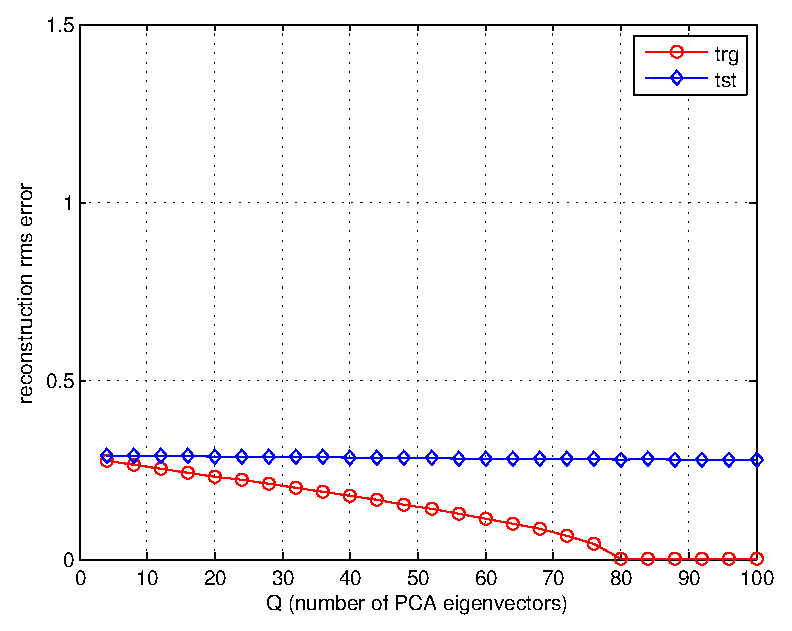
\includegraphics[width=0.25\textwidth]{figs/PCA_Uniform}}
								\subfigure[Gaussian random variable $\mathcal{N}\sim$(0, 1) in $\mathbb{R}^{1089}$, 100 realizations.]{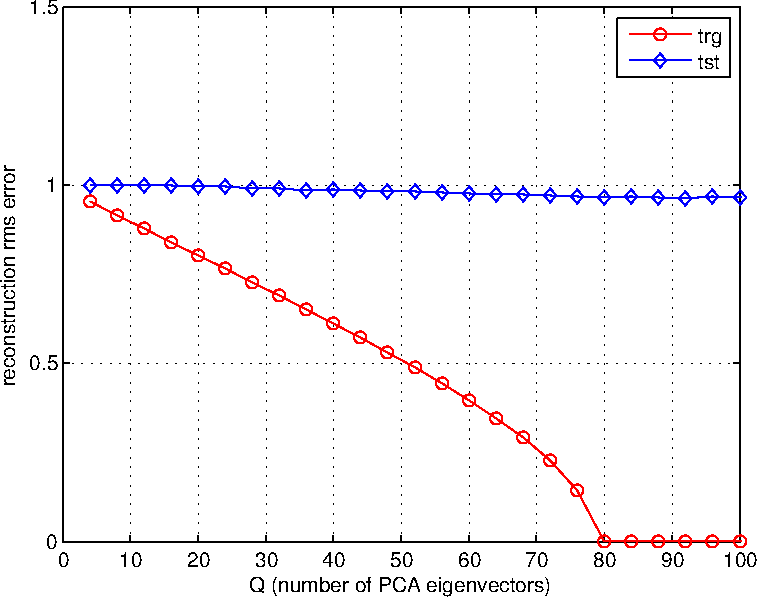
\includegraphics[width=0.25\textwidth]{figs/PCA_Gaussian}}\\
								\subfigure[Gauss-Markov random variable $\mathcal{N}\sim$(0, 1) in $\mathbb{R}^{1089}$ with 0.9 correlation, 100 realizations.]{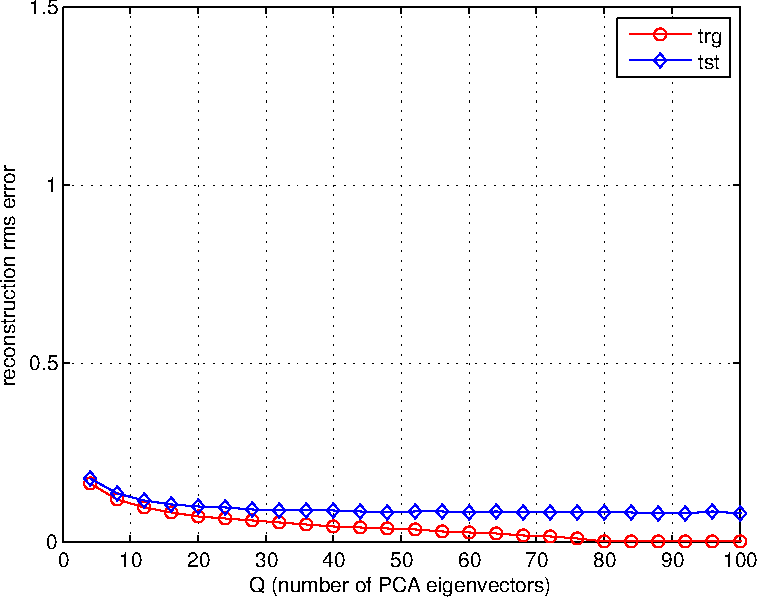
\includegraphics[width=0.25\textwidth]{figs/PCA_GaussMarkov}}
								\subfigure[Dudek sequence, 33x33 ($\mathbb{R}^{1089}$) face snippets were extracted from the first 100 images.]{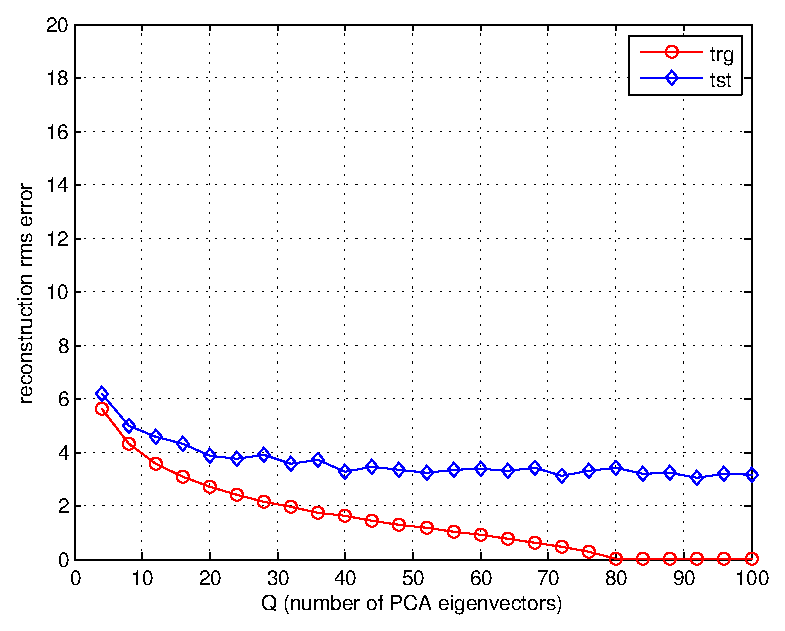
\includegraphics[width=0.25\textwidth]{figs/PCA_Dudek}}
								\caption{PCA, 100 training examples in $\mathbb{R}^{1089}$ were used for each of these experiments. Results were averaged over 10 cross-validation runs. For each run, 20\% of the data, i.e., 20 examples were randomly picked for testing while the remaining 80 examples were used for training.}
								\label{fig:PCA_results}
								\end{figure}


								\begin{figure}[t]
								\subfigure[Uniform random variable $U\sim$ \texttt{[}0, 1\texttt{]} in $\mathbb{R}^{1089}$, 100 realizations.]
								{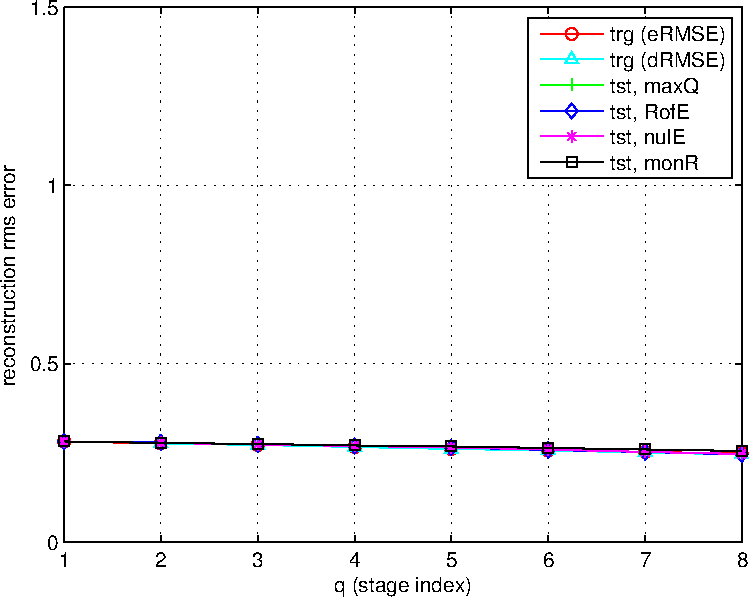
\includegraphics[width=0.25\textwidth]{figs/RVQ_8x4_Uniform}}
								\subfigure[Gaussian random variable $\mathcal{N}\sim$(0, 1) in $\mathbb{R}^{1089}$, 100 realizations.]
								{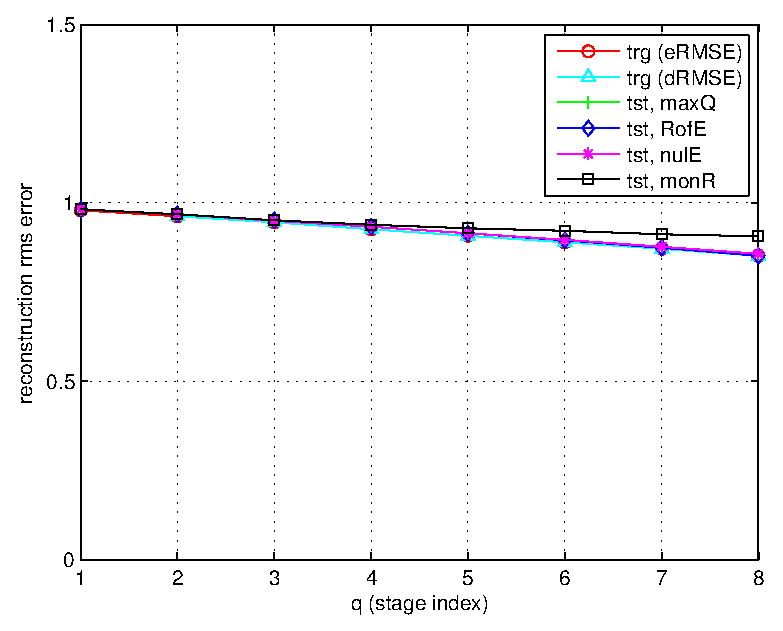
\includegraphics[width=0.25\textwidth]{figs/RVQ_8x4_Gaussian}}\\
								\subfigure[Gauss-Markov random variable $\mathcal{N}\sim$(0, 1) in $\mathbb{R}^{1089}$ with 0.9 correlation, 100 realizations.]
								{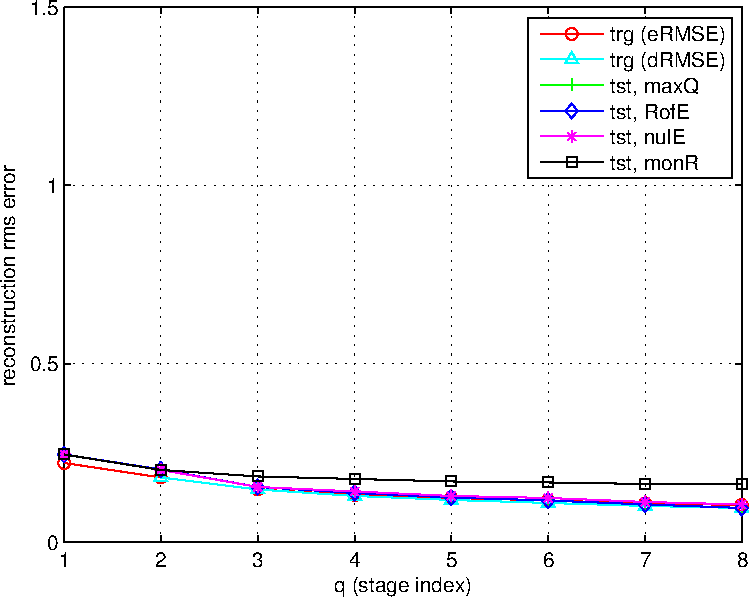
\includegraphics[width=0.25\textwidth]{figs/RVQ_8x4_GaussMarkov}}
								\subfigure[Dudek sequence, 33x33 ($\mathbb{R}^{1089}$) face snippets were extracted from the first 100 images.]
								{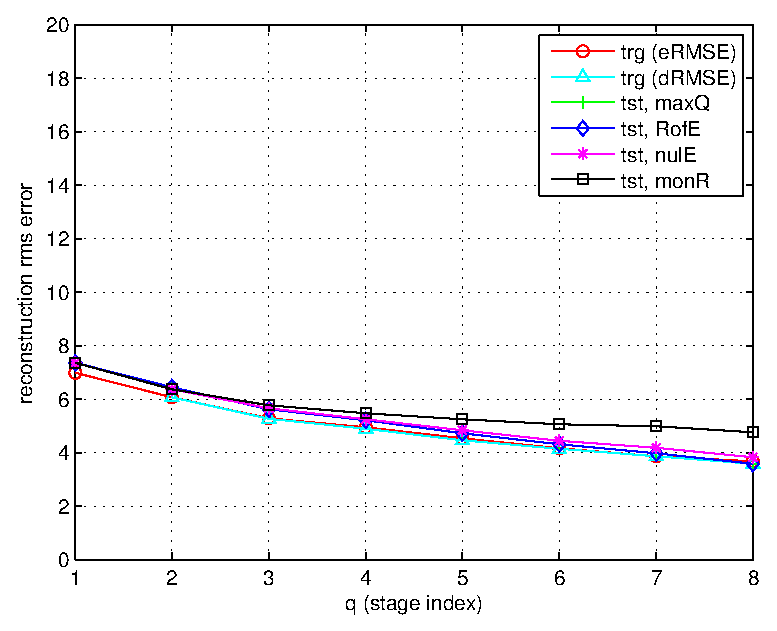
\includegraphics[width=0.25\textwidth]{figs/RVQ_8x4_Dudek}}
								\caption{RVQp, varying number of stages $P$ with number of code-vectors per stage held constant at $M=4$. 100 training examples in $\mathbb{R}^{1089}$ were used for each of these experiments. A single test example in $\mathbb{R}^{1089}$ was reconstructed.}
								\label{fig:RVQ_results_varyingP}
								\end{figure}

								
								\begin{figure}[t]
								\subfigure[Uniform random variable $U\sim$ \texttt{[}0, 1\texttt{]} in $\mathbb{R}^{1089}$, 100 realizations.]
								{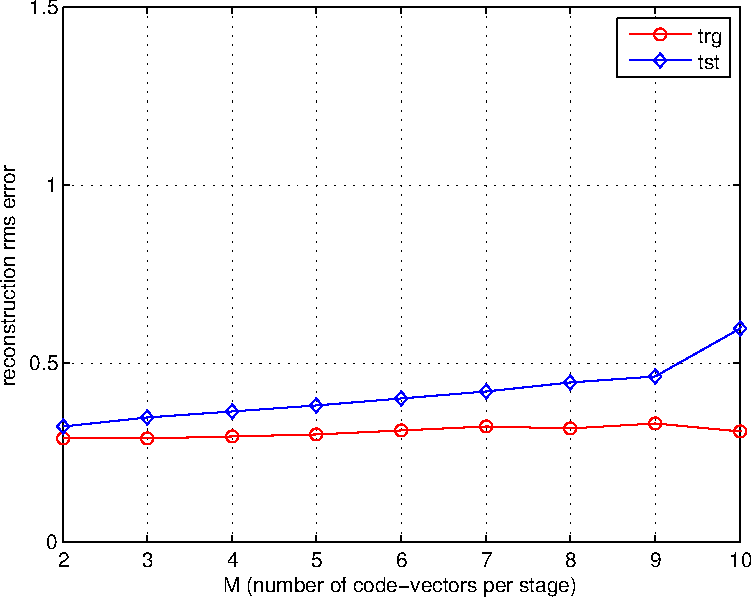
\includegraphics[width=0.25\textwidth]{figs/RVQ_uniform}}
								\subfigure[Gaussian random variable $\mathcal{N}\sim$(0, 1) in $\mathbb{R}^{1089}$, 100 realizations.]
								{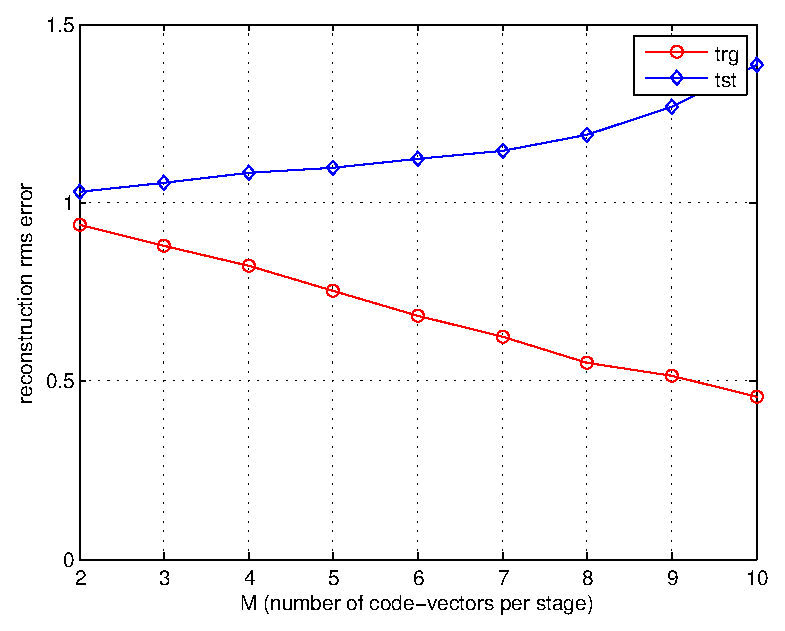
\includegraphics[width=0.25\textwidth]{figs/RVQ_Gaussian}}\\
								\subfigure[Gauss-Markov random variable $\mathcal{N}\sim$(0, 1) in $\mathbb{R}^{1089}$ with 0.9 correlation, 100 realizations.]
								{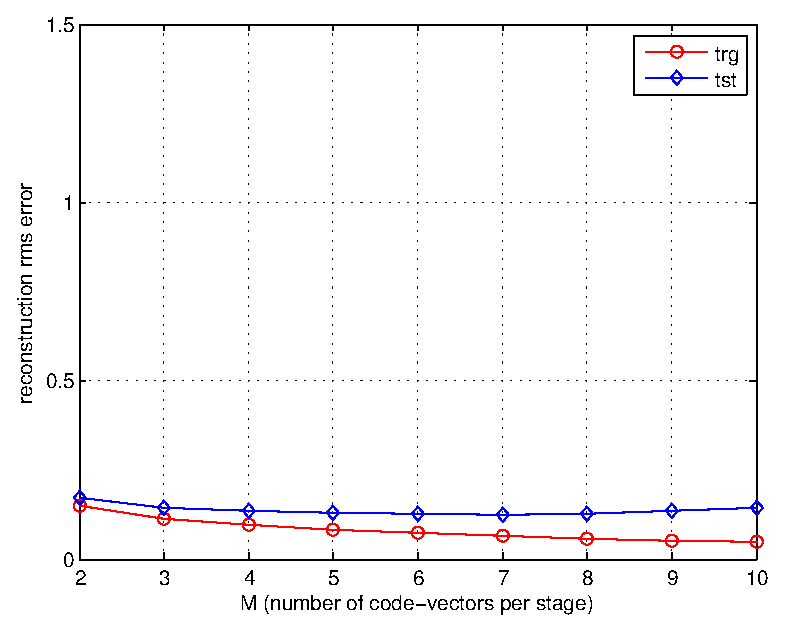
\includegraphics[width=0.25\textwidth]{figs/RVQ_GaussMarkov}}
								\subfigure[Dudek sequence, 33x33 ($\mathbb{R}^{1089}$) face snippets were extracted from the first 100 images.]
								{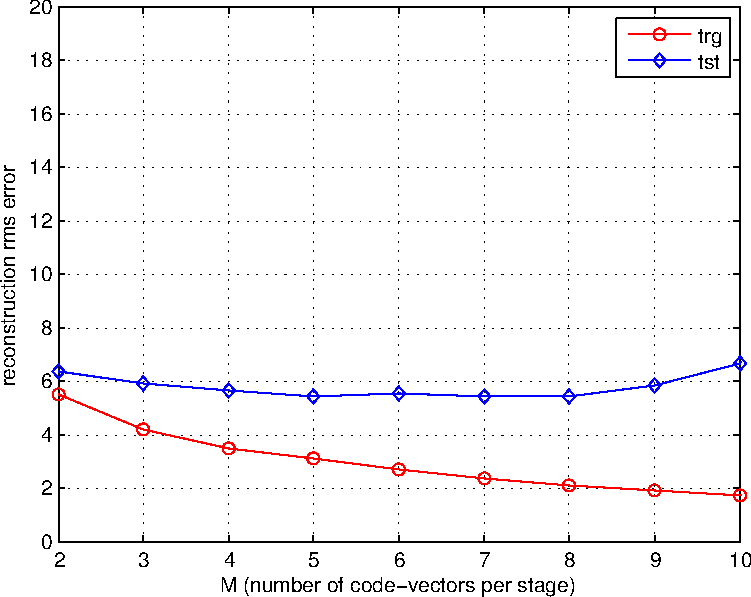
\includegraphics[width=0.25\textwidth]{figs/RVQ_Dudek}}
								\caption{RVQm, experiments, varying number of code-vectors per stage $M$ with number of stages held constant at $P=8$. 100 training examples in $\mathbb{R}^{1089}$ were used for each of these experiments. Results were averaged over 10 cross-validation runs. For each run, 20\% of the data, i.e., 20 examples were randomly picked for testing while the remaining 80 examples were used for training.}
								\label{fig:RVQ_results_varyingM}
								\end{figure}
								
								\begin{figure}[t]
								\subfigure[Uniform random variable $U\sim$ \texttt{[}0, 1\texttt{]} in $\mathbb{R}^{1089}$, 100 realizations.]{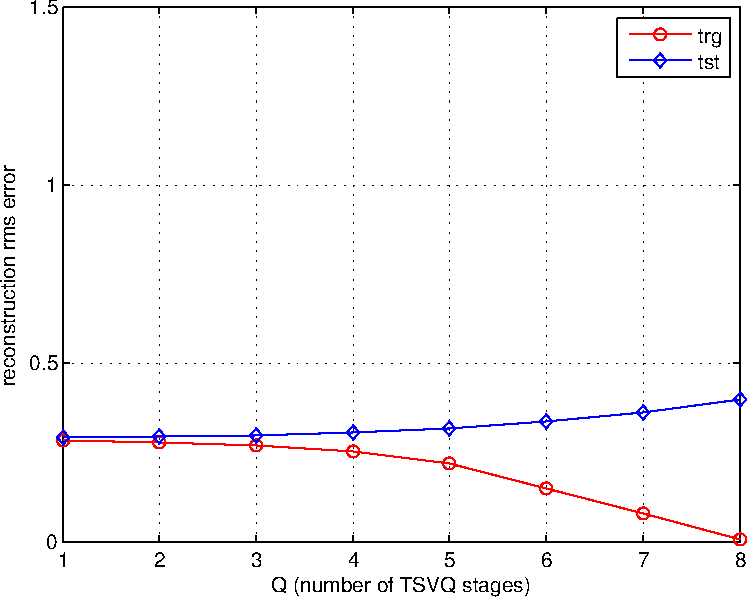
\includegraphics[width=0.25\textwidth]{figs/TSVQ_Uniform}}
								\subfigure[Gaussian random variable $\mathcal{N}\sim$(0, 1) in $\mathbb{R}^{1089}$, 100 realizations.]{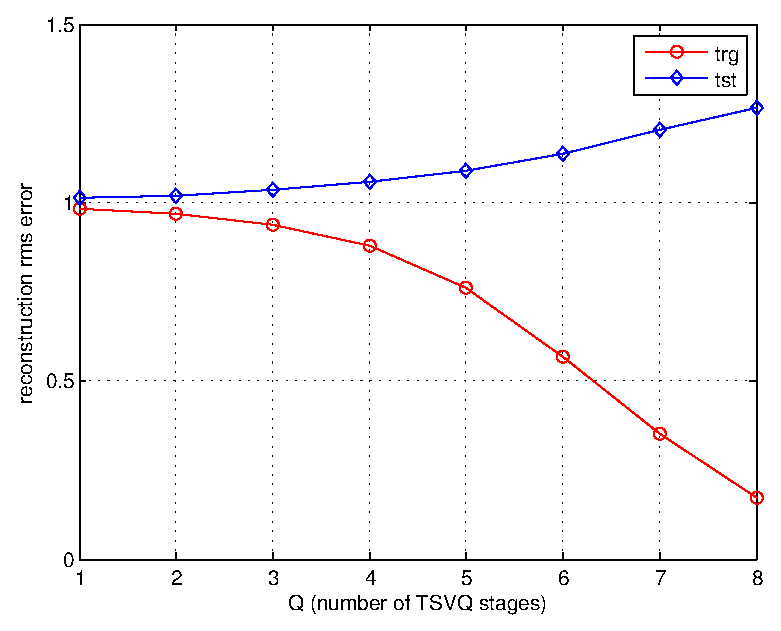
\includegraphics[width=0.25\textwidth]{figs/TSVQ_Gaussian}}\\
								\subfigure[Gauss-Markov random variable $\mathcal{N}\sim$(0, 1) in $\mathbb{R}^{1089}$ with 0.9 correlation, 100 realizations.]{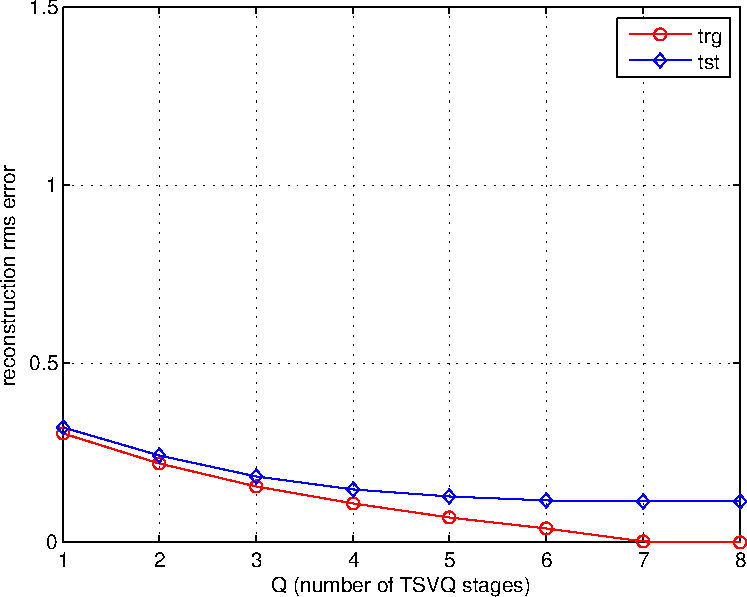
\includegraphics[width=0.25\textwidth]{figs/TSVQ_GaussMarkov}}
								\subfigure[Dudek sequence, 33x33 ($\mathbb{R}^{1089}$) face snippets were extracted from the first 100 images.]{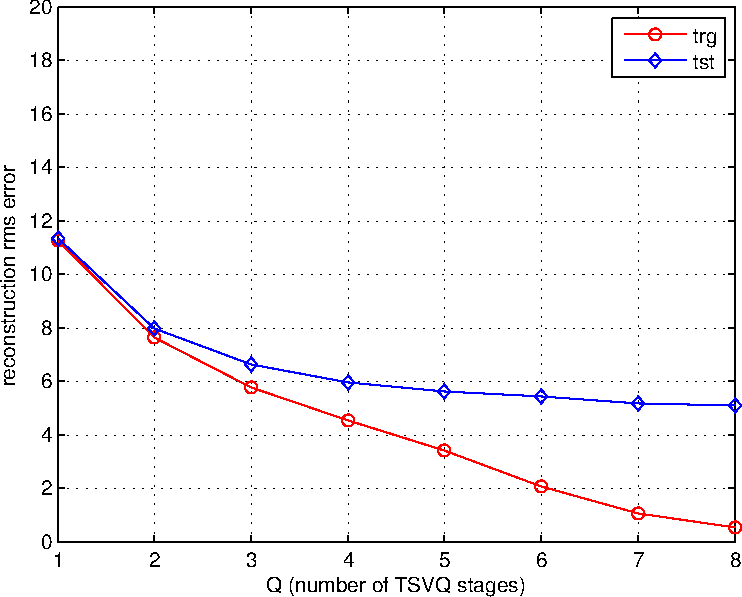
\includegraphics[width=0.25\textwidth]{figs/TSVQ_Dudek}}
								\caption{TSVQ, 100 training examples in $\mathbb{R}^{1089}$ were used for each of these experiments. Results were averaged over 10 cross-validation runs. For each run, 20\% of the data, i.e., 20 examples were randomly picked for testing while the remaining 80 examples were used for training.}
								\label{fig:TSVQ_results}
								\end{figure}

%
%								\begin{figure}[t]
%								\centering
%								\includegraphics[width=0.45\textwidth]{figs/PhD_experimentalTemporalOverview}
%								\caption{Temporal overview.}
%								\label{fig:temporal_overview}
%								\end{figure}


								\begin{figure}[t]
								\centering
								\subfigure[Best tracking error for each algorithm.]{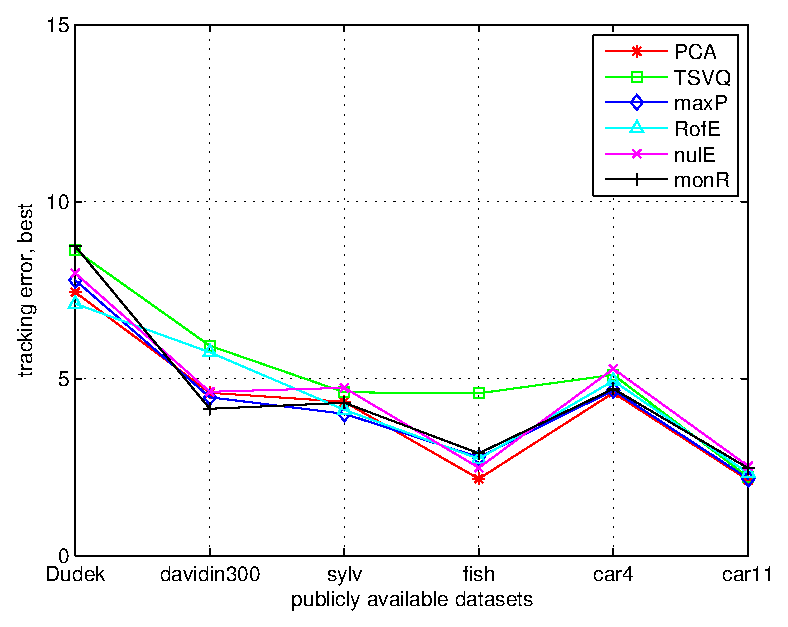
\includegraphics[width=0.23\textwidth]{figs/results_final_1a_best}\label{fig:results_final_1a_best}}
								\subfigure[\%age of datasets over which best tracking error is achieved over all parameters.]{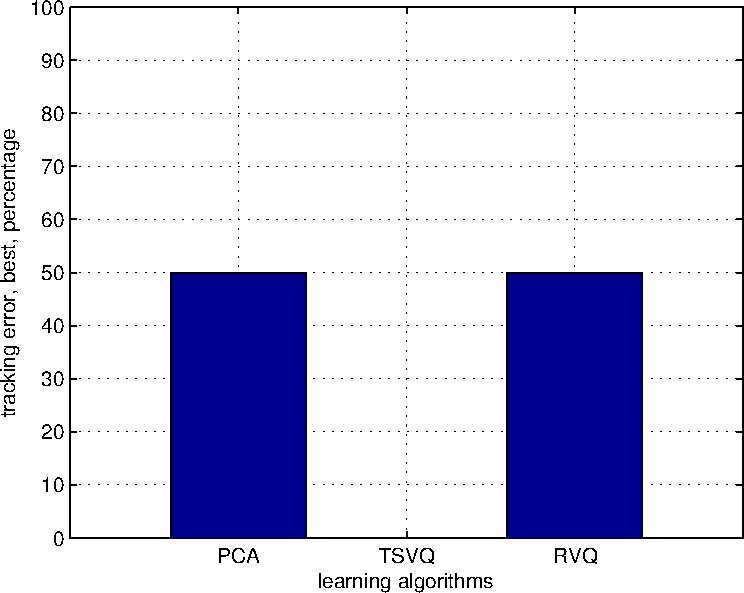
\includegraphics[width=0.23\textwidth]{figs/results_final_1b_best_percent}\label{fig:results_final_1b_best_percent}}
								\caption{Tracking results (1 of 5), comparison of best tracking performance.  PCA give best performance for half the datasets, i.e. 3 datasets, while RVQ gives best performance for the other half.}
								\label{fig:results_final_1_best}
								\end{figure}

								\begin{figure}[t]
								\centering
								\subfigure[Mean tracking error for each algorithm.]{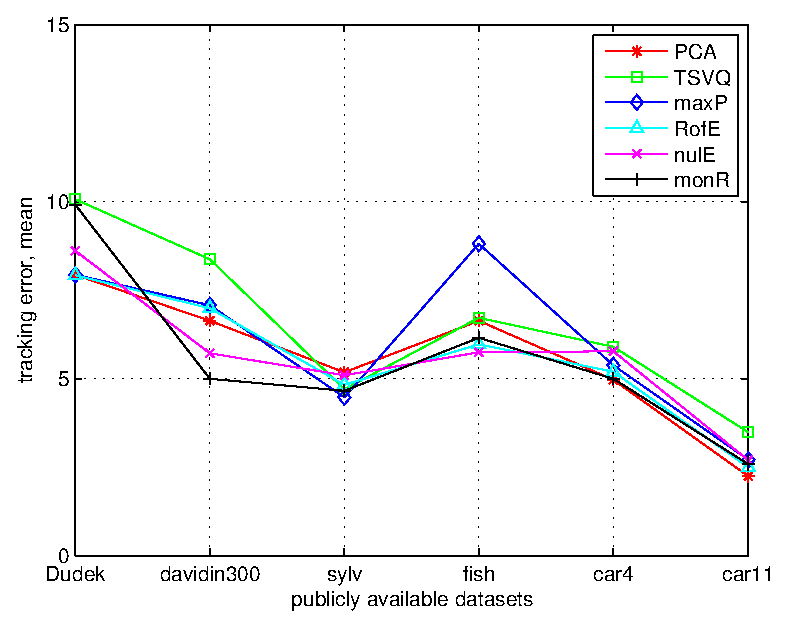
\includegraphics[width=0.23\textwidth]{figs/results_final_2a_mean}\label{fig:results_final_2a_mean}}
								\subfigure[\%age of datasets over which best mean tracking error is achieved over all parameters.]{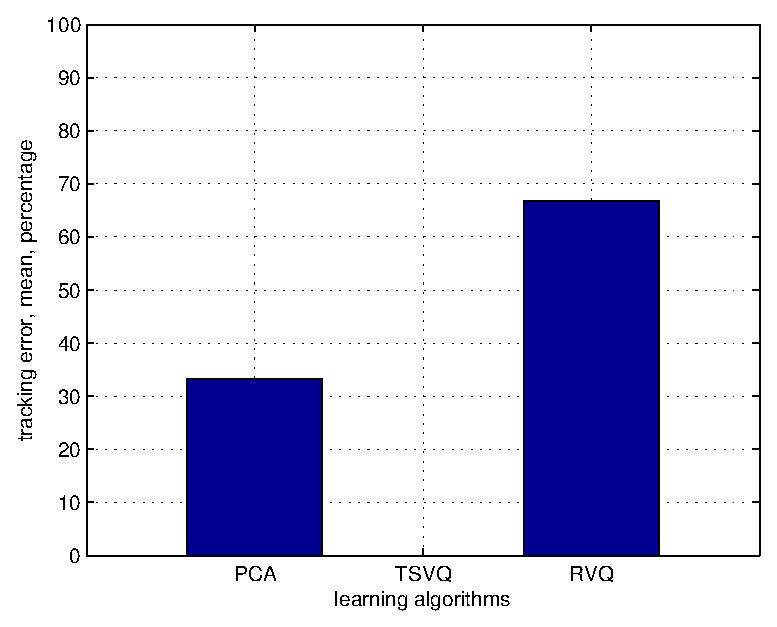
\includegraphics[width=0.23\textwidth]{figs/results_final_2b_mean_percent}\label{fig:results_final_2b_mean_percent}}
								\caption{Tracking results (2 of 5), comparison of mean tracking performance.  RVQ performs better over twice as many datasets as PCA.}
								\label{fig:results_final_2_mean}
								\end{figure}

								\begin{figure}[t]
								\centering
								\subfigure[Tracking error for each algorithm with 16 eigenvectors/code-vectors stored in memory.]{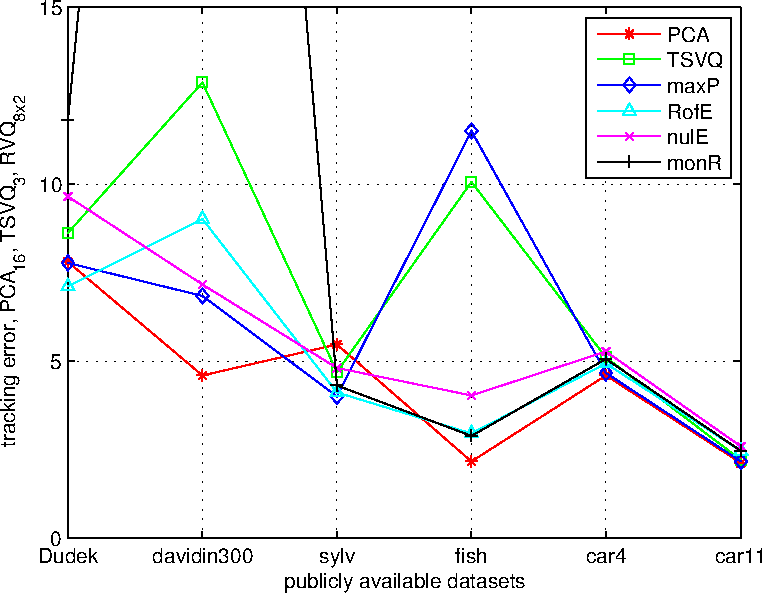
\includegraphics[width=0.23\textwidth]{figs/results_final_3a_16}\label{fig:results_final_3a_16}}
								\subfigure[\%age of datasets over which best tracking error is achieved with 16 eigenvectors/code-vectors stored in memory.]{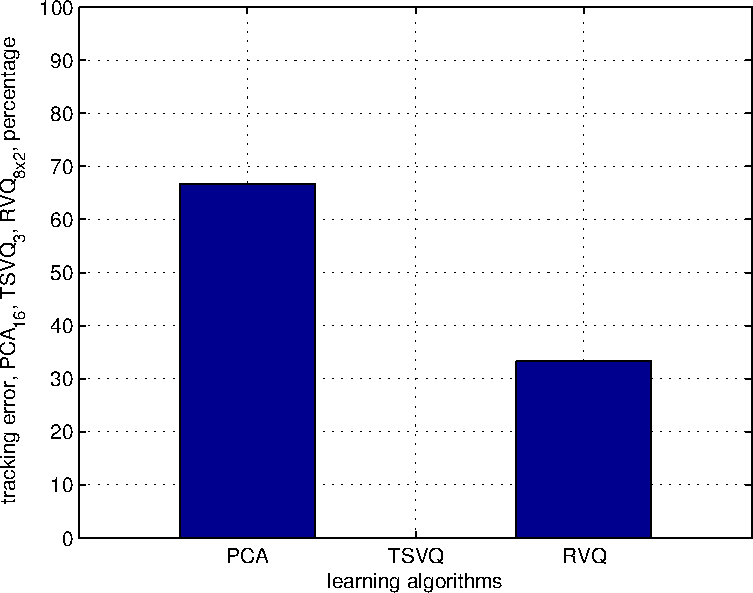
\includegraphics[width=0.23\textwidth]{figs/results_final_3b_16_percent}\label{fig:results_final_3b_16_percent}}
								\caption{Tracking results (3 of 5), comparison of tracking performance if 16 eigenvectors/code-vectors are stored in memory.  PCA performs better over twice as many datasets as RVQ.}
								\label{fig:results_final_3_16}
								\end{figure}

								\begin{figure}[t]
								\centering
								\subfigure[Tracking error for each algorithm with 32 eigenvectors/code-vectors stored in memory.]{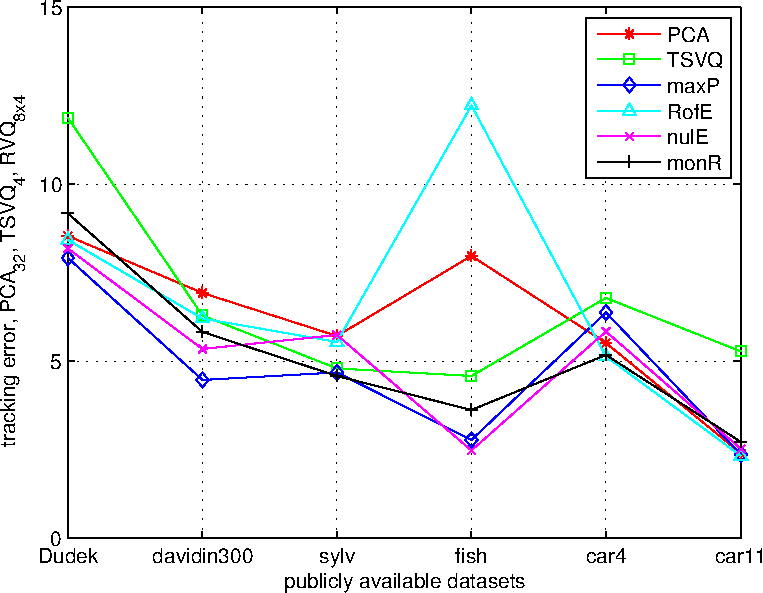
\includegraphics[width=0.22\textwidth]{figs/results_final_4a_32}\label{fig:results_final_4a_32}}
								\subfigure[\%age of datasets over which best tracking error is achieved with 32 eigenvectors/code-vectors stored in memory.]{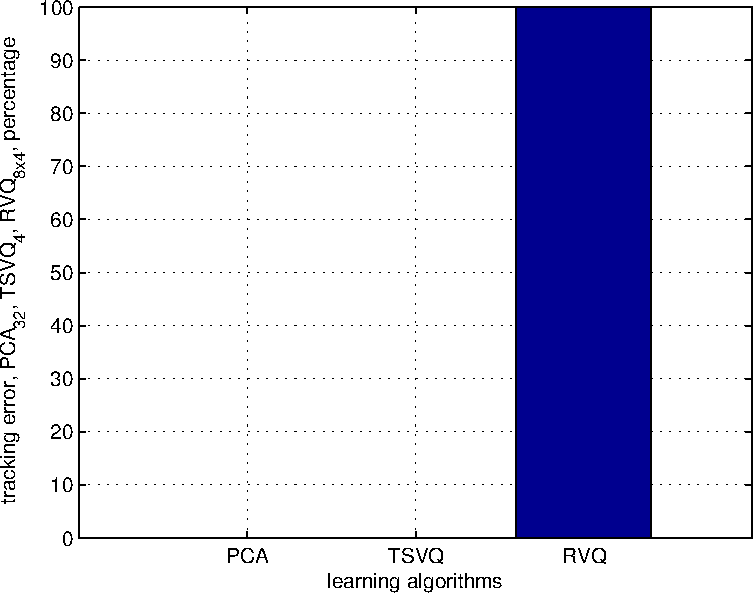
\includegraphics[width=0.22\textwidth]{figs/results_final_4b_32_percent}\label{fig:results_final_4b_32_percent}}
								\caption{Tracking results (4 of 5), comparison of tracking performance if 32 eigenvectors/code-vectors are stored in memory.  RVQ performs the best over all datasets.}
								\label{fig:results_final_4_32}
								\end{figure}

								\begin{figure}[h!]
								\centering	
								\subfigure[PCA]{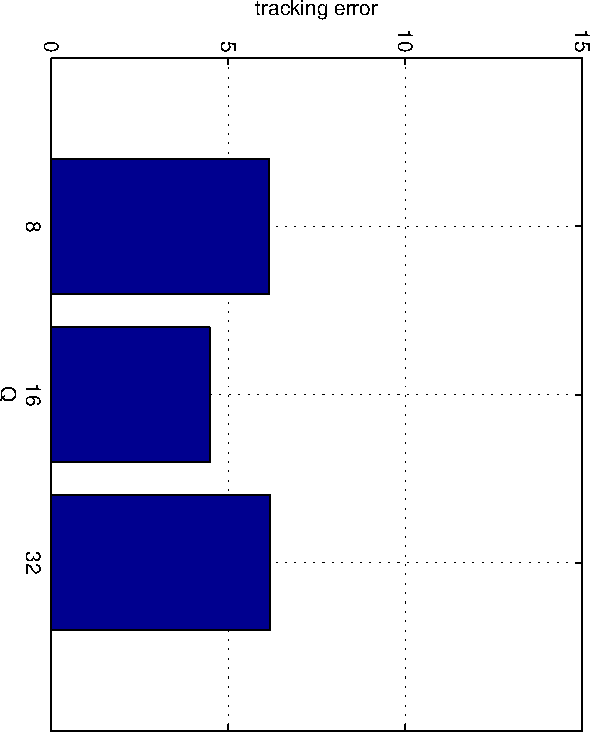
\includegraphics[width=0.17\textwidth, angle=90]{figs/results_final_5a_pca_}\label{fig:results_final_5a_pca_}}
								\subfigure[TSVQ.]{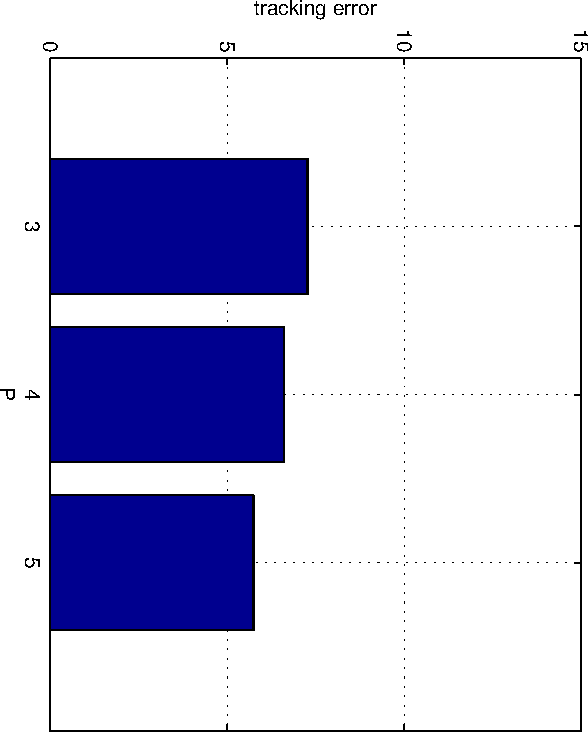
\includegraphics[width=0.17\textwidth, angle=90]{figs/results_final_5b_tsvq}\label{fig:results_final_5b}}
%								\subfigure[maxP.]{\includegraphics[width=0.22\textwidth]{figs/results_final_5c_maxP}\label{fig:results_final_5c}}
%								\subfigure[RofE.]{\includegraphics[width=0.22\textwidth]{figs/results_final_5d_RofE}\label{fig:results_final_5d}}
%								\subfigure[nulE.]{\includegraphics[width=0.22\textwidth]{figs/results_final_5e_nulE}\label{fig:results_final_5e}}
%								\subfigure[monR.]{\includegraphics[width=0.22\textwidth]{figs/results_final_5f_monR}\label{fig:results_final_5f}}
								\subfigure[maxP, RofE, nulE, monR.]{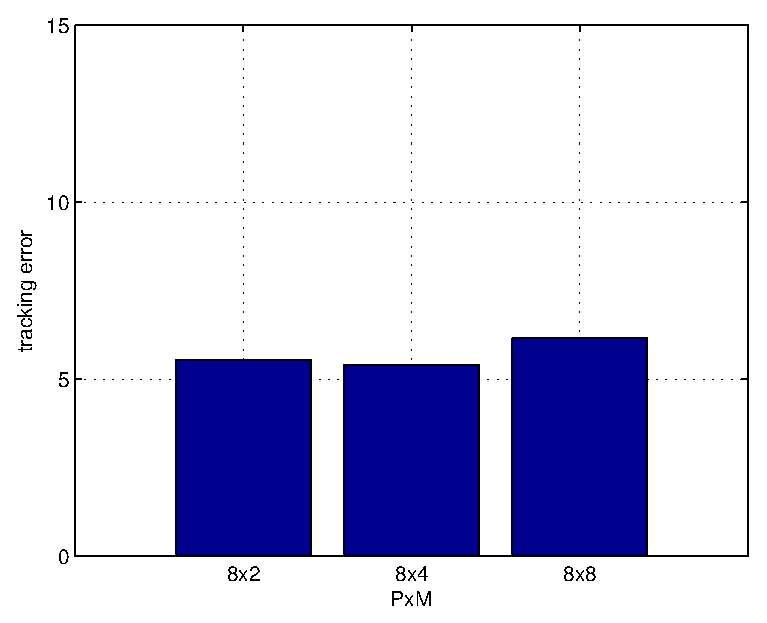
\includegraphics[width=0.22\textwidth]{figs/results_final_5g_8x2_8x4_8x8}\label{fig:results_final_5g_8x2_8x4_8x8}}
								\caption{Tracking results (5 of 5), comparison of tracking performance as parameters for each algorithm are varied.  In (d), we see that over all RVQ algorithms, RofE has best mean performance.  In (g) it is clear that the best RVQ configuration is 8x4.}
								\label{fig:results_final_5_configs}
								\end{figure}

We now turn to the second component of our framework, visual tracking.

%==========================	
\section{SUBSPACE BASED TRACKING}
%==========================
One of the main factors limiting visual tracking is the lack of suitable appearance models~\cite{2003_JNL_TRKsubspace_Jepson}.  In subspace based tracking, the basic assumption is that the evolving target appearance can be modeled using a lower dimensional subspace computed using Principal Components Analysis (PCA), or a few code-vectors computed using a VQ based method, such as RVQ.  This approach has several advantages such as compact representation (only a few basis eigenvectors or stage code-vectors are needed to capture variations in the target appearance), continuous model update, less offline training data requirement, no need for optimization and a possible pre-processing step for object recognition.  A disadvantage of this approach is that the tracker is prone to drift if the online appearance model is updated incorrectly. 

In order to classify or recognize complex articulated objects, a large range of appearances is required.  One approach has been to use interpolation of appearance from a small number of views~\cite{1991_JNL_Recog_Ullman}, storing a fixed number of views that suffice for the application at hand~\cite{1992_JNL_VBR_Breuel}, incremental adding of views~\cite{1993_CNF_Gestures_Darrell}, storage of basis sets~\cite{1996_TRK_region_Hager}, and affine-warping based eigentracking~\cite{1998_JNL_Eigentracking_Black}.  A fundamental issue in eigentracking is whether to create one eigenspace for all classes or one eigenspace per class.  This is addressed in~\cite{1997_JNL_EigenTRK_Moghaddam} in which the classes correspond to $M$ human head orientations with $N$ examples in every class.  In a \emph{parametric} eigenspace, one eigenspace is created for all $NM$ images.  On the other hand, in a \emph{view-based} eigenspace, one eigenspace is created for each of $M$ head orientations, each with $N$ users per eigenspace.  Since multiple views of a face form a connected non-convex region~\cite{1994_JNL_FaceTop_Bichsel}, the analogy of using a parametric versus a view-based eigenspace approach is that of modeling a complex distribution by a single cluster model or the union of several component clusters respectively.  It is shown that the latter approach will give better image reconstruction results~\cite{1997_JNL_EigenTRK_Moghaddam}.  In our work, we use the former approach since we currently deal with single-target tracking.  This issue will however be addressed in future work in multi-target tracking.

Recently, a tracker based on online updating of a PCA eigenspace was presented by Ross et. al. in~\cite{2008_JNL_subspaceTRK_Ross}.  In this work, the authors use incremental PCA with observation weighting and a particle filter to build an online incremental basis.  It is assumed that observations are generated from this eigenspace.  In this context, it is shown in~\cite{2008_JNL_TRKsubs_Skocaj} that the squared reconstruction error degradation is less than 10\% when using the incremental PCA update algorithm versus using the optimal batch PCA algorithm.  Also,~\cite{2010_CNF_TRKsubs_Qian} use an approach quite similar to that used in~\cite{2008_JNL_subspaceTRK_Ross}.  They sample a collection of image patches and likelihood of each image patch is generated by reconstruction.  Comparison is made between PCA subspace tracking with and without weighting prior observations.  They show that temporal weighting the data results in less background clutter penetrating the target of interest and therefore leads to better occlusion handling in tracking.  In our work, we do not use weighting since there is no known computationally efficient method of data weighting for RVQ.  To keep our results fair, we do not use data weighting for PCA and TSVQ based tracking either.  


%====================
\section{EXPERIMENTS}
%====================
In this section, we combine information on RVQ and tracking methods presented in the previous two sections into a visual tracking framework using RVQ and compare it with visual tracking using PCA and TSVQ.  All trackers were run on 6 publicly available datasets, Dudek, davidin300, sylv, fish, car4 and car11.  These datasets can be downloaded from~\cite{2008_JNL_subspaceTRK_Ross}. Tracking error was measured on each of these datasets using the error between manually selected ground truth interest points and the estimates produced by our algorithms.  The approach we take in this work builds on work presented by Ross et. al. in 2008~\cite{2008_JNL_subspaceTRK_Ross}.  We have used part of their software with their permission~\cite{2008_SFT_Ross}.  In this spirit, we make our own software available for download at \mbox{{\url{https://github.com/SalmanAslamPhD/PhD}}}.  

Our goal is to produce estimates at every time frame of the target state.  In order to accomplish this, our tracking framework is based on five components: (a) target representation, (b) target motion, (c) appearance model, (d) observation model, and (e) target inference.  

First, the goal of the representation model is to provide a means of specifying a target.  Several target representation methods are described in~\cite{2006_JNL_SURVEYtrk_Yilmaz}.  We use the bounding quadrilateral method.  This quad encloses the pixels of a target of interest.  It is also allowed to warp affinely from frame to frame to minimize inclusion of background pixels as the target changes shape, size and orientation.

Second, the goal of the motion model is to specify the motion that the target is expected to follow.  In order to keep our work general, we do not assume any deterministic target motion model.  The target is expected to move according to a Wiener process, i.e., brownian motion.  An advantage of this approach is that arbitrary camera and target motion are allowed.  A disadvantage of this approach in the context of the particle filter is that particles need to be evaluated all around the current target position, rather than around a predicted target position in a certain direction.  We are therefore unable to take advantage of the reduced spatial search-space that comes with a deterministic motion model.  At time $t$, the goal of the tracking process is to estimate the well-known affine state vector $\mathbf{X}_t = (\theta, \lambda_1, \lambda_2, \phi, x, y)$.  To keep our model as general as possible, all 6 components of the state vector are modeled as Gaussian random variables but with known variance which is specified in the first frame.  However, in order to simplify sampling from the joint density, it is possible to use certain relaxation criteria such as Markovian dependence which allows factoring the joint density into a product of conditional densities, or independence, which allows factoring into individual prior densities.  We choose the latter to avoid MCMC sampling and note that this method works well in practice.  The target motion is therefore represented not in analytic form but as a 6x6 diagonal covariance matrix $\Sigma_X$ centered at the state vector $\mathbf{X}_{t-1}$ in the previous frame.  The elements on the diagonal represent variances of the affine parameters, $\sigma_\theta^2, \sigma_{\lambda_1}^2, \sigma_{\lambda_2}^2, \sigma_\phi^2, \sigma_x^2, \sigma_y^2$.  For instance, for the $x$ and $y$ coordinates of the target at time $t$, the probability of the target position is given by $p(x_t|x_{t-1}) = \mathcal{N}(x_{t-1}, \sigma_x^2)$ and $p(y_t|y_{t-1}) = \mathcal{N}(y_{t-1}, \sigma_y^2)$.  At every time step, predicted values are sampled from all 6 distributions.  Each predicted set is used to warp a zero-centered grid onto or around the target of interest.  
%Next, we discuss the inference model which is used to select the best set of affine candidates generated by the motion model.

Third, the goal of the appearance model is to provide a compact representation of the target's pixel intensities.  In this work, we use a learned eigenspace for PCA, a trained $\sigma$-tree codebook for RVQ and a binary balanced-tree codebook for TSVQ.  In order to understand appearance modeling, we conduct the following 4 experiments using PCA, RVQ and TSVQ to measure rms errors for target reconstruction: (a) PCA, varying number of eigenvectors, $Q$, (b) RVQp, varying number of stages $P$ for RVQ while holding the number of code-vectors per stage constant at $M=4$, (c) RVQm, varying number of code-vectors per stage $M$ for RVQ while holding the number of stages constant at $P=8$, and (d) TSVQ, varying number of stages, $P$.  It is hoped that investigating reconstruction errors will aid in understanding the behavior of these various algorithms when used to model target appearance in tracking applications.  We use four datasets in $\mathbb{R}^{1089}$: (a) Uniform random variable, (b) Gaussian random variable, (c) Gauss-Markov random variable, and (d) images from the Dudek sequence. The reason for using $\mathbb{R}^{1089}$ is that our targets for all our tracking datasets are warped to a canonical size of 33-pixel height and 33-pixel width (33x33=1089). In all cases, we take 100 examples and split them up using an 80/20 rule, i.e. 80 training examples and 20 test examples. 10 cross-validation runs are used. In each cross-validation run, the training and test examples are picked randomly in the 80/20 ratio.  Results for PCA, RVQp, RVQm and TSVQ are shown in Figures~\ref{fig:PCA_results}, \ref{fig:RVQ_results_varyingP}, \ref{fig:RVQ_results_varyingM} and \ref{fig:TSVQ_results} respectively.  We make several observations from these figures.  The first set of observations regards training error.  Training error is always less than test error, as expected.   For PCA and RVQp, monotonic decrease in rms reconstruction error with increasing $Q$ and $P$ is observed respectively as expected, since both algorithms rely on successive approximation. For PCA, training error becomes 0 when $Q=80$ since there are 80 training examples.  For TSVQ and RVQm, monotonic decrease or approximately constant rms reconstruction error with increasing $P$ and $M$ respectively is observed.  This is also expected since both these algorithms rely not on successive approximation but on populating the decision space with code-vectors and maximizing inter-cluster distance in the process.  The second set of observations regards test error.  In this context, we see that for the uniform and Gaussian random variables, test error for PCA and RVQp stays almost constant with increasing $Q$ and $P$ respectively.  The reason is that PCA and RVQp use successive refinement when increasing $Q$ and $P$ respectively.  Test error is therefore not expected to get better since it is not possible to better explain random data with increasing $Q$ and $P$.  For RVQm and TSVQ, test error increases with increasing $M$ and $P$ respectively.  For TSVQ, increasing $P$ controls its VC (Vapnik-Chervonenkis) dimension~\cite{1999_BOOK_PRML_Vapnik} and therefore its generalization ability~\cite{2003_JNL_PRML_Karacali}.  It appears that increasing $M$ in RVQm has a similar effect.  The reason is that with $P=1$, increasing $M$ in RVQ is equivalent to increasing $P$ in TSVQ.  Increasing $P$ in RVQ adds additional refinement to the equivalent code-vectors but $M$ controls the overall general placement of RVQ code-vectors in the decision space $\mathbb{R}^D$.  Therefore, in RVQ, it is $M$ more than $P$ that controls generalization ability.  Therefore, when $M$ in RVQm or $P$ in TSVQ increase, their generalization ability decreases , leading to better explanation of training data, but with less ability to explain the test data well. For both RVQm and TSVQ, notice that when training error falls off sharply, test error increases sharply. Also, when training error drop is gradual, so is test error increase rate. This confirms over-training behavior. Also, RVQ increase or decrease rates are more gradual than TSVQ.  The reason is that for RVQm, the number of equivalent code-vectors increase as $2^8, 3^8, 4^8, \ldots, 10^8$.  Even for small values of $M$, the number of equivalent code-vectors is already quite large.  For TSVQ, the terminal code-vectors increase as $2^1, 2^2, 2^3, \ldots, 2^8$ and therefore there is a rapid increase in the number of code-vectors from a very small value to a very large value.  Finally, the rms reconstruction error is lower for uniform random data than for Gaussian random data.\footnote{It may be tempting to explain this using an entropy argument.  The uniform distribution has the maximum entropy among all continuous distributions with finite support $[a,b]$ while the Gaussian distribution has maximum entropy among all distributions with infinite support~\cite{1982_JNL_MaxEntropy_Jaynes}.  However, due to the difference in support, it is difficult to compare entropies.} The reason is that the variance of the Gaussian distribution is 1 while the variance of the uniform distribution with support $[0,1]$ is much lower at 1/12~\cite{1993_BOOK_RandomProcesses_Garcia}.  For the Gauss-Markov and Dudek cases, all 4 algorithms display decreasing test error with increasing $Q$ or $P$. The leveling off of the test error, or the "knee-point"~\cite{2009_BOOK_PRML_Escolano}, is visible in all cases.  In these experiments, we see that training error of PCA is in general better than RVQ. This is expected since PCA can achieve perfect reconstruction when $Q$ comes close to the number of training examples $N$, $N<<D$.  Test errors however are comparable.  RVQ has 2 knobs, $P$ and $M$. In varying $P$, it acts like PCA in providing successive approximation. In varying $M$, it acts like TSVQ in changing its VC dimension, and therefore its generalization ability.  Given this flexibility, it is expected that RVQ will perform well in our tracking framework.

Fourth, the goal of the observation model is to (a) generate observations based on the motion and representation model outputs, and (b) generate a likelihood score for each observation using the appearance model.  For PCA, the likelihood of a target observation is assumed proportional to the DFFS (distance to feature space).  For RVQ, the likelihood of a target observation is assumed to be proportional to the Euclidean distance to a direct-sum code-vector reached through sequential search.  We use two methods, \emph{maxP} and \emph{RofE}, to compute the full-stage direct-sum code-vectors, and two methods, \emph{nulE} and \emph{monR} to compute the partial-stage direct-sum code-vectors. An observation model $p(z_t|x_t)$ relates the state $x_t$ at time $t$ to the observation $z_t$ at time $t$.  The observation model generates observations that will serve as candidates for the target and then assigns scores to each candidate.  For PCA, it is assumed that an image $\mathbf{x}$ in $\mathbb{R}^D$ is probabilistically generated from a subspace $\mathbf{U}$ spanned by earlier observed images.  The covariance matrix $\Sigma$ of the input training images can be written as $\Sigma = \mathbf{U}\mathbf{\Lambda} \mathbf{V}^T$.  Here $\mathbf{\Lambda}$ is the matrix of eigenvalues.  The distribution is assumed to be Gaussian centered at $\boldsymbol{\mu}$.  The probability of an image being generated under this distribution is inversely proportional to its distance from $\boldsymbol{\mu}$.  This distance can be decomposed into two parts.  The first is DFFS (distance-from-feature-space).  In a partial KL expansion using $Q$ eigenvectors, the space spanned by these $Q$ eigenvectors is given by $\mathbf{F}$\footnote{We use $\mathbf{U}$ interchangeably with $\mathbf{F}$ here.  Whereas the notation $\mathbf{U}$ is more widely used to represent a PCA eigenspace, we use $\mathbf{F}$ to remain compatible with~\cite{1997_JNL_EigenTRK_Moghaddam}.} and the signal residual $\epsilon^2$ is given by $\epsilon^2 = \Vert \tilde{\mathbf{x}} \Vert^2 - \sum\limits_{i=1}^Q \mathbf{u}_i^2 = \sum\limits_{i=Q+1}^D \mathbf{u}_i^2$, where $\tilde{\mathbf{x}}$ is the mean removed input image and $\mathbf{u}_i$ are the eigenvectors of the covariance matrix estimate, $\boldsymbol\Sigma=\tilde{\mathbf{x}}\tilde{\mathbf{x}}^T$  .  This signal residual is referred to as DFFS.  The second is DIFS (distance-in-feature-space), the component of $\mathbf{x}$ which lies in the feature space $\mathbf{F}$.  In a Gaussian distribution, the probability of a data point $\mathbf{x}$ in $\mathbb{R}^D$ depends on the Mahalanobis distance $d$.  The output of PCA, zero-centered $\mathbf{\tilde{y}}$ is decorrelated with variances along each dimension equal to the eigenvalues $\lambda_i$ of the covariance matrix $\boldsymbol\Sigma$.  This formulation, first presented in~\cite{1997_JNL_EigenTRK_Moghaddam} shows that the first term in the sum is the DIFS term while the second term corresponds to DFFS.  With this formulation, PCA can be used in a probabilistic framework since the error of a test vector $\mathbf{x}$ now also depends on its distance from the mean of the data.  However, as mentioned in~\cite{2008_JNL_subspaceTRK_Ross}, it is difficult to weight these two terms.  In this work, we therefore only use DIFS so that our approach does not rely on finding different weights for different datasets.  As mentioned earlier, VQ, like PCA, does not define a proper density in the observation space~\cite{1999_JNL_Gaussian_roweis}.  However, it is common to assign a probability measure to a new data point in proportion to the distance of the closest centroid~\cite{1999_JNL_Gaussian_roweis}, $p(\mathbf{x}_i|\boldsymbol\mu_k) = \frac{e^{-\big(\dr\big)}} {\sum\limits_{i=1}^N e^{-\big(\dr\big)}}$.  Here, $\boldsymbol\mu_k$ is the closest code-vector to test data-point to $\mathbf{x}_i$,  $P_{\textrm{max}}$ is the number of stages in the codebook, $P_i$ is the number of stages required to decode $\mathbf{x}_i$, and $\lambda$ is a regularization parameter.  We use 4 different RVQ methods to compute which $\boldsymbol \mu_k$ input data-point $\mathbf{x}_i$ maps to: (a) maxP in which RVQ decoding is carried out so that maximum stages $P$ are used, (b) RofE, in which realm of experience coding is used, i.e., a test vector is decoded such that the decode path traversed belongs to the set of training decode paths, (c) nulE, in which null encoding is used, i.e. reconstruction rms error is checked at every stage and a stage is skipped if at that stage, rms error is not reduced, and (d) monR, in which monotonic rms error is a condition which if not met results in a halt in the decoding  process.  In our tracking framework, we use all 4 methods above and compare their performance. 

Fifth and finally, the goal of the inference model is to: (a) weight the likelihoods of various observations and make a decision on which observation should be picked as an estimate for the target position and appearance, and (b) keep a temporal record of which observations were not picked in the previous frames as best estimates but may still potentially be considered in future frames.  In tracking, the correspondence of observations in the current frame to existing targets in the previous frame is generally an ill-posed problem~\cite{2005_CNF_TRK_Yang}.  We use the particle filter to deal with this problem by propagating multiple hypotheses from frame to frame~\cite{1998_JNL_Condensation_IsardBlake}.  The computational complexity of this method does not grow with frames as opposed to the multi-hypofigs2 tracker (MHT)~\cite{1993_JNL_SURVEYcorresp_Cox}.

These models work together to produce state estimates at every time frame.  The motion model and the representation model work together to generate 600 affine parameter sets as candidates for the target state.  The observation model takes these affine parameter sets and extracts observations, i.e., candidate window-chips, also called \emph{snippets}~\cite{2007_JNL_IDDM_Barnes} from the image.  It then uses the appearance model to generate a likelihood score for each snippet.  Finally, the inference model picks the snippet with the highest score and goes through a resampling step so that snippets with low likelihood scores are eliminated.  The affine parameters of the resampled snippets are then given to the motion model in the next frame and the process continues.  The inference model makes the final decision of which candidate snippet to pick as the target.  Our inference model makes no assumption of linearity or Gaussianity.  What this means is that we do not assume that the motion or observation models are linear, nor do we assume that the likelihood of finding a target at a particular location has a Gaussian distribution.  Morever, we would like to keep a history of possible target candidate states, 600 in this case, so that soft decisions can be made about the target state at each frame.  In other words, at every frame, even though we make a decision as to which particular snippet best represents the target, we acknowledge that this decision could be erroneous and therefore we propagate other candidates through time.  This allows us to revisit candidate snippets that were not picked in previous frames as the target estimate but that could still have a high probability of being the correct snippet.  Also, we do not want our hypotheses to grow with time.  Keeping all this in mind, we base our inference model on the sequential Monte Carlo (SMC) filter, i.e., the particle filter~\cite{2002_JNL_PF_Arulampalam}.  

%--------------------------------------------------------------------------------------------------------------------------------------------------------------
\section{RESULTS}
%--------------------------------------------------------------------------------------------------------------------------------------------------------------
We now present tracking error results for 6 different trackers, PCA-based, TSVQ-based and 4 RVQ-based trackers, maxP, RofE, nulE, and monR.  We start with Figure~\ref{fig:results_final_1_best}.  In this figure, we plot best possible tracking performance for each algorithm.  For PCA, this means the best possible performance attained for each of the datasets for number of eigenvectors $Q$=8, 16 and 32.  For TSVQ, best possible performance for each dataset is over number of stages $P$=3, 4 and 5.  For maxP, RofE, nulE and monR, best possible performance for each dataset is over number of stages $P$ and number of codevectors $M$, $PxM$=8x2, 8x4 and 8x8.  The reason for plotting performance for each dataset separately is that each dataset represents a different distribution and we would like to gauge performance for each algorithm over the different distributions.  We see that performance for PCA and all 4 RVQ based algorithms is very close while TSVQ tracking error is highest in many cases.  PCA performs best in the fish, car4 and car11 sequences while RVQ performs best in the remaining three datasets, Dudek, davidin300 and sylv.  TSVQ does not perform best in any sequence.  Note that the performance difference between PCA and RVQ in the car4 and car11 sequences is negligible.  Recall that car4 and car11 are relatively benign datasets with little variation in pose and lighting.  The fish sequence has sudden motion as well as sudden global lighting changes.   Since global lighting change induces linear correlation in the data, it makes sense that PCA does well in this sequence.  The reason is that global illumination changes move the illuminated object within the modeled PCA subspace~\cite{1987_JNL_Faces_Sirovich}.  RVQ performs best over the Dudek, davidin300 and sylv sequences.  All 3 of these sequences have moderate lighting changes while Dudek and davidin300 have several forms of noise as discussed earlier.  For Dudek, RofE does best.  The reason is that in the presence of uncertainties, RofE holds tight to what has already been modeled and is resistant to accepting sudden changes in the underlying distribution.  It is therefore better able to handle blur and other forms of noise that do not exist in the training data.  On the other extreme is monR which greedily attempts to minimize reconstruction error.  Out of all RVQ methods, this method performs worse, but even then, not by much.  Second best performance is for maxP which is again not a greedy method.  Third best performance is for nulE which is also a greedy method but less so than monR.

We now turn to Figure~\ref{fig:results_final_2_mean}.  In this figure, mean performance over all parameters is shown.  It may be noted that monR loses track in one instance.  That instance is not factored into the means since it is not clear how penalize a lost track when performing mean computations.  Here, we see that RVQ performs best 66.7\% of the time.  This time, in addition to Dudek, davindin300 and sylv, RVQ performs better than PCA in the fish sequence as well.  The reason for this is that PCA is unable to track the fish sequence well when it has too few, i.e., 8 eigenvectors or when it has too many, i.e., 32 eigenvectors.  In the 8 eigenvector case, the subspace does not have enough dimensions to model lighting changes well.  Even though it has been shown, as mentioned earlier, that only 3 eigenvectors are needed to model lighting changes~\cite{1987_JNL_Faces_Sirovich}, in practice this does not hold due to shadowing and specularities~\cite{1997_JNL_EigenVsFisherFaces_Bel}.  For too many eigenvectors, over-fitting is an issue.  For $Q=16$, PCA performs best and that is why it had best possible performance.  However, when it comes to means, all 4 RVQ parameters are able to outperform PCA in mean performance.  In Figure~\ref{fig:results_final_3_16}, we hold the number of eigenvectors for PCA or codevectors for TSVQ and RVQ constant at 16 (actually 14 for TSVQ but we ignore this slight difference).  In these figures, we see that PCA outperforms RVQ for 16 vectors.  In Figure~\ref{fig:results_final_4_32}, we hold the number of eigenvectors for PCA or codevectors for TSVQ and RVQ constant at 32 (actually 30 for TSVQ but we ignore this slight difference).  In these figures, we see that RVQ completely outperforms PCA for 32 vectors.  The reason is that at $8x4$, RVQ now has enough capacity to explain the underlying distributions, and is better able to do so than PCA or TSVQ.  Finally, in Figure~\ref{fig:results_final_5_configs}, we plot mean tracking performance over all datasets for each algorithm.  Here we see that PCA performs best for $Q=16$, while both RofE and monR have best mean performance over all parameters and over all datasets.  Moreover, over all RVQ configurations, 8x4 performs best when averaged over all datasets.

%--------------------------------------------------------------------------------------------------------------------------------------------------------------
\section{CONCLUSIONS}
%--------------------------------------------------------------------------------------------------------------------------------------------------------------
In this work, we have demonstrated successful application of RVQ for visual tracking over a variety of datasets, and compared our results with PCA and TSVQ based tracking.  We have based our design on a well-known method for visual tracking so that our newer RVQ based tracking method can be compared easily with existing methods in the literature.  Overall, PCA and RVQ outperform TSVQ completely.  Between PCA and RVQ, RVQ outperforms PCA in more areas.  It appears that in a tracking scenario, it is more useful to model a target using its centroids rather than to try to solve the more difficult problem of generating its subspace under limited data conditons.  

Our next step is to explore multiple targets, multi-spectral inputs, comparison with non-linear manifold learning methods such as LLE (locally linear embedding) and MDS (multidimensional scaling), using higher stage refinement for RVQ, and an investigation into the relation of RVQ with PCA using the subspace based approach given in~\cite{2004_CNF_KmeansVsPCA_DingHe}.


\bibliographystyle{IEEE}
\bibliography{MyCitations}

\end{document}
